\documentclass[12pt]{article}
\usepackage{amsmath} % flere matematikkommandoer
\usepackage[utf8]{inputenc} % æøå
\usepackage[T1]{fontenc} % mere æøå
\usepackage[danish]{babel} % orddeling
\usepackage{verbatim} % så man kan skrive ren tekst
\usepackage[all]{xy} % den sidste (avancerede) formel i dokumentet
\usepackage{graphicx}

\title{ProjektKursus Systemudvikling 2014\\Delrapport 2}
\author{}

\begin{document}
\maketitle
Gruppemedlemmer:\\
Kenneth Christensen: 02 08 93\\Michael Jensen: 01 07 93\\Rune Pedersen: 01 11 82\\Rasmus Hansen: 03 12 92
\\\\
Instruktør: Kasper Passov

\pagebreak
\section{Abstract}
Vi har valgt at udarbejde et projekt for  ”BMX-Butikken”, det er en butik der har specialiseret sig indenfor BMX sporten, som er placeret i københavn.  De sælger alt indenfor BMX, som indebærer alt fra tøj og sko, til cykler og dele. Udover en fysisk butik på nørrebrogade, har bmxbutikken også en online webshop som ligger på www.bmxbutikken.dk.
Projektet går ud på at lave en applikation til smartphones. Denne skal hjælpe bmx kørerer med at finde nye steder at køre på, som før var forbeholdt de lokale, derudover vil applikationen også vise  brugerne hvor bmx-butikken ligger og eventuelle samarbejdspartnere.
Ideen med applikationen er at den skal appelere til bmx kørere, dette kan både være lokale som vil udforske deres by yderligere, eller folk fra andre dele af landet på besøg i København samt såkaldte bmx eller skate turister. Applikationen Vil hovedsageligt dreje sig om københavnsområdet.
Vi vil bygge appen ved hjælp af programmerings sproget JAVA og bruge værktøjer som "android developer tools".

\section{IT-projektets formål og rammer}
Følgende model er en FACTOR analyse af projektet og giver en kort og konkret beskrivelse af rammerne for projektet.
\begin{figure}[h]
    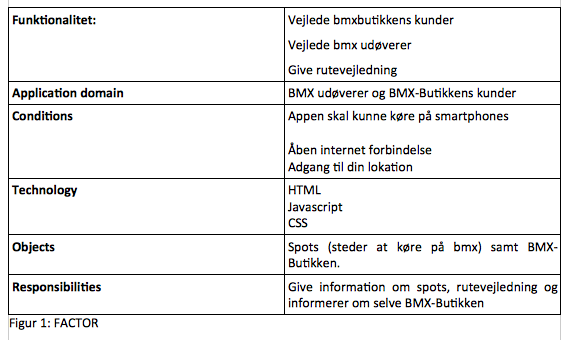
\includegraphics[scale=0.5]{factor.png}
\end{figure}

\pagebreak

\section{Kravspecifikation for IT-løsningen}
Følgende punkter:\\
(a) De funktionelle og ikke-funktionelle krav til jeres system\\\\
Funktionelle krav:\\
Upload af billeder\\
Mulighed for at kommenterer\\
Menu\\
Streetspots\\
Skatesparks\\
Markers\\
Rutevejledning\\
Bruger lokation\\
Rating system\\
Mulighed for at oprette sig som bruger\\
BMX-Butikken\\\\
Ikke funktionelle krav:\\
Appens sprog skal være på engelsk\\
Bruger venligt UI\\\\
(b) En use case model, der beskriver system-funktionaliteten. Der ønskes et højniveau-diagram,
som giver overblik over hvilke use cases de forskellige aktører har.\\
(c) Tre specificerede use cases, som er særlig vigtige i jeres system, se fx OOSE figur 4-22.\\
(d) Et klassediagram over jeres problemområde (solution-domain).\\
(e) Sekvens-diagrammer over de 3 use-cases specificeret i punkt (c).\\
Husk at alle diagrammer skal være fulgt af tekstbeskrivelser, der gør diagrammerne fuldt
forståelige også for læsere uden særligt domænekendskab.

\section{Systemdesign sammenfatning}
Kapitlet resumerer jeres foreløbige system-design så kort og klart som muligt. Samtidig
udpeger I de vigtigste udestående design- og implementationsopgaver.

\section{Program- og systemtest}
Dokumenter jeres foreløbige test af IT-løsningen. I kapitlet sammenfattes hovedresultaterne af
jeres test-aktiviteter; mens test plan, test case specification, test incident report og test report
summary placeres som bilag.


\section{Brugergrænseflade og interaktionsdesign}
(a) Præsenter skærmbilleder af de mest interessante dele af jeres brugergrænseflade.\\
(b) Illustrer flowet/dynamikken i brugerinteraktionen mellem skærmbillederne.\\
(c) En audio-visuel præsentation af brugergrænsefladen af den seneste kørende prototype.\\
Formatet vælger I frit, fx en video der illustrerer IT-løsningen med vigtige use cases, en serie
screenshots med speak, slideshow med forklarende tekst. Dog skal det i alle tilfælde afleveres som
et YouTube link og være uploadet som en ”skjult video”.\\
(d) Resultatet af seneste tænke-højt forsøg gennemført med een eller flere af jeres brugere.


\section{Versionstyring}
Til aflevering: Som bilag skal vedlægges jeres nuværende commit-log samt jeres
programkode. Kommentér kort (ca 1/2 side) de vigtigste ændringer, der er sket i programkoden.

\section{Projektsamarbejdet}
Til aflevering: Beskriv konkret og oplysende hvordan det går med samarbejdet med brugerne
og med arbejdet internt i gruppen. Herunder skal bl.a. oplyses antallet af møder med brugerne under
projektforløbet (fx på en tidslinje), mødeformen i gruppen, samt hvorledes jeres referat- og
dokumentationsform fungerer. Hvorledes prioriterer og styrer I projektindsatsen, så I sikrer
fremdrift på de felter, som er mest risikable/afgørende for et succesfuldt resultat? Herunder, beskriv
og diskuter:\\
(a) Hvad går godt?\\
(b) Hvad går mindre godt?\\
(c) Hvad vil I gøre for at effektivisere jeres udviklingsarbejde?

\pagebreak
\section{Review}
\subsection{Designing for usability}
Artiklen omhandler metoder for en programmør til at fuldfører IT-projekter, der ender ud med at have en høj værdi af "usability" (Nemt og intuitivt for slutbrugeren at benytte). Det handler primært om 3 teoretiske systemudviklings metoder, som ophavsmændene til artiklen mener man bør følge for at udvikle et nemt og brugbart computer system. De 3 metoder er: "Early and continual focus on users", "empirical measurement of usage" and "iterative design". \\\\
Early and continual focus on users\\
Handler om at designerne skal forstå hvem slutbrugerne er. Det betyder at designerne skal studere brugernes arbejde og evaluerer på hvordan bruger interagere med systemet.\\\\
Empirical measurement of usage\\
Går ud på at der i udviklings processen skal indlægges tid til at lave slutbruger undersøgelser. Konkret betyder det at der i processen skal udvikles prototyper, som slutbrugeren kan benytte til at udføre deres faktiske arbejde. Brugeren skal så observeres og processen skal analyseres for at forbedre prototypen.\\\\
Iterative design\\
Går ud på at når brugerne finder en fejl under en test, skal fejlene udbedres. Det betyder så at produktet skal igennem en ny design fase, testing, "measurement". Disse 3 faser gentages så ofte som dette måtte være nødvendigt for at opnå det ønskede niveau af funktionalitet, brugervenlighed og hvad man ellers måtte prioritere.
\\\\
Resten af artiklen omhandler disse 3 teoretiske metoder i forhold til virkeligheden. Der lægges vægt på at de nævnte metoder virker intuitive for en programmør/designer når de bliver læst højt, men flere tests viser at metoderne måske ikke er så intuitive alligevel. Undersøgelsen viser nemlig at meget få mener at netop disse metoder er nogle af de hovedpunkter man skal overveje når man skal udvikle og evaluere et nyt system. Derudover sammenlignes denne protokol også med andre som "get it right, the first time" og deciderede design guidelines. \\\\
Konkret bliver det pointeret at det er stortset umuligt at "get it right the first time", det ville nemlig indebære at der var blevet lavet et perfekt systemdesign fra starten, samt at man ignorede eventuelle erfaringer man gjorde sig om brugeren og systemet undervejs i projektet. Generelle guidelines ses som værende ufuldstændige og problematiske. Hvilket kommer af at design guidelines netop er generelle og altså ikke tager højde for nogen konkrete situationer der måtte opstå og derfor kommer designeren til at skulle træffe de fleste beslutninger selv.\\\\
Det vi i gruppen mener der er værd at tage med fra denne artikel er selve ideen om at gøre et system brugervenligt, nemt og intuitivt. Vi er enige om at et gennemført system der er nemt at bruge, er et system der i højere grad vil blive brugt. For at trække paraleller til vores eget projekt, så har vi indtil videre kun været i tæt dialog omkring funktionalitet med vores kunde og ikke snakket meget om selve systemets interface. Dermed må vi også erkende at selvom metoderne nu virker intuitive, oplagte og at netop disse metoder er blevet prædiket flere gange til forskellige forelæsninger, endda i forskelle fag. Så er metoderne alligevel ikke kommet intuitivt og vi må derfor bestræbe os på at få en dialog igang med nogle slutbrugere, der kan evaluere på vores foreløbige systemdesign og måske forbedre det. På den måde kan vi implementere de 3 metoder og få gang i en "design, test og evaluerings" cyklus og løbende forbedre vores system imens vi nærmer os et slutprodukt.\\\\


\end{document}

